\documentclass[11pt,a4paper]{article}
\usepackage[margin=1in]{geometry}
\usepackage[T1]{fontenc}
\usepackage[utf8]{inputenc}
\usepackage{lmodern}
\usepackage{hyperref}
\usepackage{enumitem}
\usepackage{xurl}
\usepackage{tikz}
\usepackage{float}
\usetikzlibrary{arrows.meta, positioning, shapes.geometric}
\hypersetup{colorlinks=true,linkcolor=blue,urlcolor=blue}
\newcommand{\codepath}[1]{\path{#1}}
\tikzset{box/.style={rectangle,draw,rounded corners,align=center,inner sep=3pt,minimum width=36mm},line/.style={-Latex}}

\title{Phase-2 gem5: Deliverable 3 (Adapter Contract)}
\author{Senior Systems Architecture}
\date{\today}

\begin{document}
\maketitle

\section{Technical Description}
This deliverable enforces contract conformance for gem5: adapter emits normalized intervals; engine consumes contract-only data.

\section{Implementation Fulfillment}
Reference contract is documented in \codepath{Phase-2/ADAPTERS.md}; schema validation is implemented in \codepath{Phase-2/ingest/ingest_api.py}; gem5 implementation is \codepath{Phase-2/adapters/gem5_adapter.py}.

\section{Design \& Architecture}
Contract boundary:
\begin{itemize}[leftmargin=*]
  \item Allowed in adapter: parse, normalize, infer state/residency, validate schema.
  \item Forbidden in adapter: window policy, SIT equation, summary/export semantics.
\end{itemize}
This preserves target extensibility and deterministic behavior under shared engine logic.

\subsection*{Function Flowchart}
\begin{figure}[H]
\centering
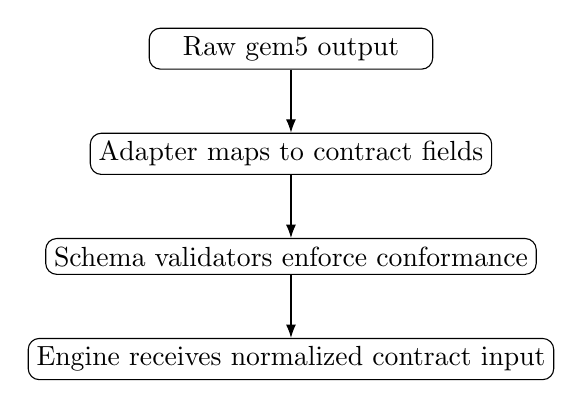
\begin{tikzpicture}[node distance=8mm and 12mm]
\node[box] (a) {Raw gem5 output};
\node[box, below=of a] (b) {Adapter maps to contract fields};
\node[box, below=of b] (c) {Schema validators enforce conformance};
\node[box, below=of c] (d) {Engine receives normalized contract input};
\draw[line] (a) -- (b);
\draw[line] (b) -- (c);
\draw[line] (c) -- (d);
\end{tikzpicture}
\caption{gem5 Contract Conformance Flow}
\end{figure}

\end{document}
